\subsubsection{Nitretação Gasosa}
Para a simulação com condições de contorno dadas para a nitretação gasosa foram utilizados os parâmetros vistos na Seção \ref{sec:param-gas}, além daqueles comuns dados pela Tabela \ref{tab:resumoParametros}. Os valores de $\Delta t$ e $\Delta x$ utilizados foram 0,01s e 0,1 $\mu m$, para um tempo total de 22 horas e 35 $\mu m$ de profundidade, com temperatura igual a 718K.

Os resultados mostrando a concentração de nitrogênio em função da profundidade ao longo do tempo para a simulação com concentração superficial variável, para nitretação gasosa, estão representados nas Figuras \ref{fig:csvar-gas1} e \ref{fig:csvar-gas2}.

\begin{figure}[!htb]
\centering
	\caption{Resultado da simulação da Segunda Lei de Fick para concentração na superfície variável, considerando nitretação a gás, até 2 horas}
	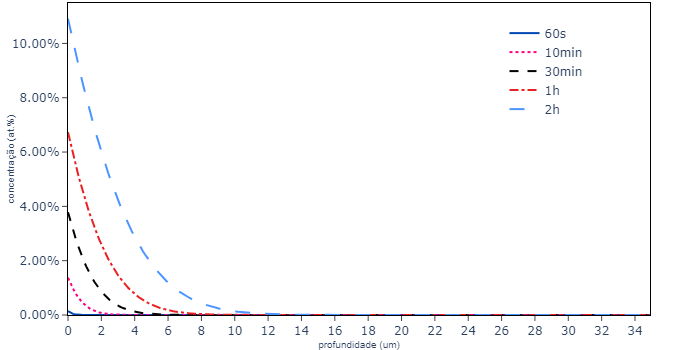
\includegraphics[width=1.0\textwidth]{plot_fickGas}
	\label{fig:csvar-gas1}
	\centering
	\fonte{Elaborado pela autora}
\end{figure}

Na Figura \ref{fig:csvar-gas2} estão também representados os dados experimentais do artigo \cite{christiansen2008nitrogen}. No artigo, o experimento foi realizado com aço AISI 316,  à 440°C, durante 23 horas, com potencial de nitretação de 1,41 $bar^{-1/2}$. 

\begin{figure}[!htb]
\centering
	\caption{Resultado da simulação da Segunda Lei de Fick para concentração na superfície variável, considerando nitretação a gás, até 22 horas, com resultado experimental de \cite{christiansen2008nitrogen}}
	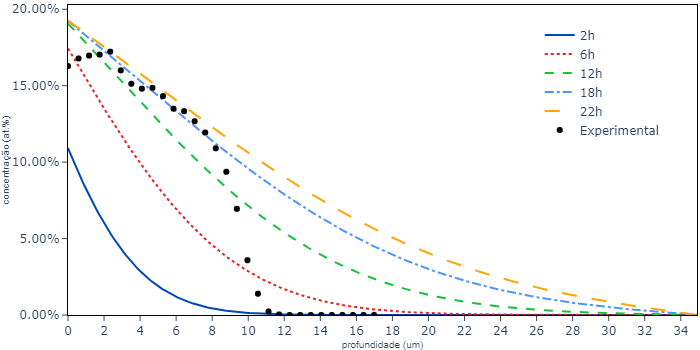
\includegraphics[width=1.0\textwidth]{plot_fickGasExp}
	\label{fig:csvar-gas2}
	\centering
	\fonte{Elaborado pela autora}
\end{figure}


\FloatBarrier


\subsubsection{Nitretação a Plasma}
Para a nitretação a plasma aplicada à Segunda Lei de Fick, foram utilizados os parâmetros 
da Tabela \ref{tab:resumoParametros}, a corrente média igual a 0,44mA/cm$^2$, $H_0$=7,29 $\times 10^{28} m^{-3}$ e $H_{superficie}$=1,6$\times$ 10$^{22} m^{-2}$ (este último obtido pelo melhor \textit{fit}). Os valores de $\Delta t$ e $\Delta x$ utilizados foram 0,01s e 0,1 $\mu m$, para um tempo total de 22 horas e 35 $\mu m$ de profundidade, com temperatura igual a 718K.

O resultado experimental para uma nitretação a plasma, obtido de \cite{moskalioviene2011modeling}, corresponde a um experimento realizado em aço AISI 316L, à 400°C, durante 2 horas.

Os resultados mostrando a concentração de nitrogênio em função da profundidade ao longo do tempo para a simulação considerando nitretação a plasma estão representados nas Figuras \ref{fig:csvar-plasma1} e \ref{fig:csvar-plasma2}. Os dados experimentais mencionados anteriormente estão visíveis na Figura \ref{fig:csvar-plasma1}.


\begin{figure}[!htb]
\centering
	\caption{Resultado da simulação da Segunda Lei de Fick para concentração na superfície variável, considerando nitretação a plasma, até 2 horas com resultados experimentais retirados do artigo de \cite{moskalioviene2011modeling}}
	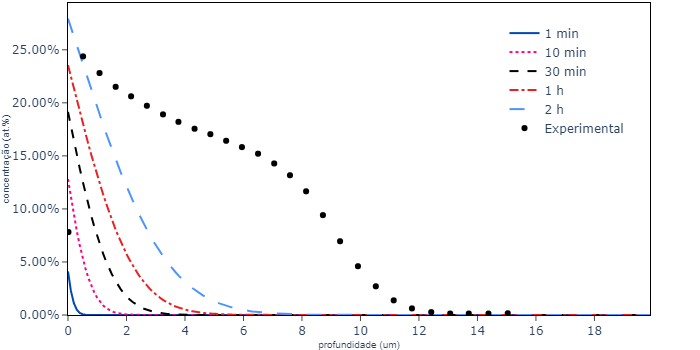
\includegraphics[width=1.0\textwidth]{plot_fickPlasmaExp}
	\label{fig:csvar-plasma1}
	\centering
	\fonte{Elaborado pela autora}
\end{figure}

\begin{figure}[!htb]
\centering
	\caption{Resultado da simulação da Segunda Lei de Fick para concentração na superfície variável considerando nitretação a plasma, até 22 horas}
	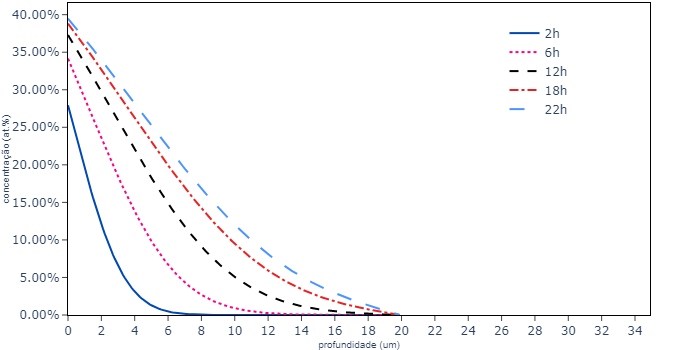
\includegraphics[width=1.0\textwidth]{plot_fickPlasma2}
	\label{fig:csvar-plasma2}
	\centering
	\fonte{Elaborado pela autora}
\end{figure}

\FloatBarrier